The $9$ last experiments we made have two goals : displaying the non-unicity of the global minima and finding the influence of the population size, especially in terms of solution unicity.\\
\\
\emph{For the following experiments, $\sigma=2$, $\frac{U{add}}{\widetilde{F}}=2.5\% $, $U^{mul}=50\% $ and we limit the number of BeATS evaluations to $3000$.} \\
\\
Fig. \ref{fig:lambdacp}. shows the exact same result quality for every execution with common parameters and for every $\lambda$ value.\\
\begin{figure}[!h]
	\caption{Congestion pattern matching plots : evolution with $\lambda$.}
	\label{fig:lambdacp}
	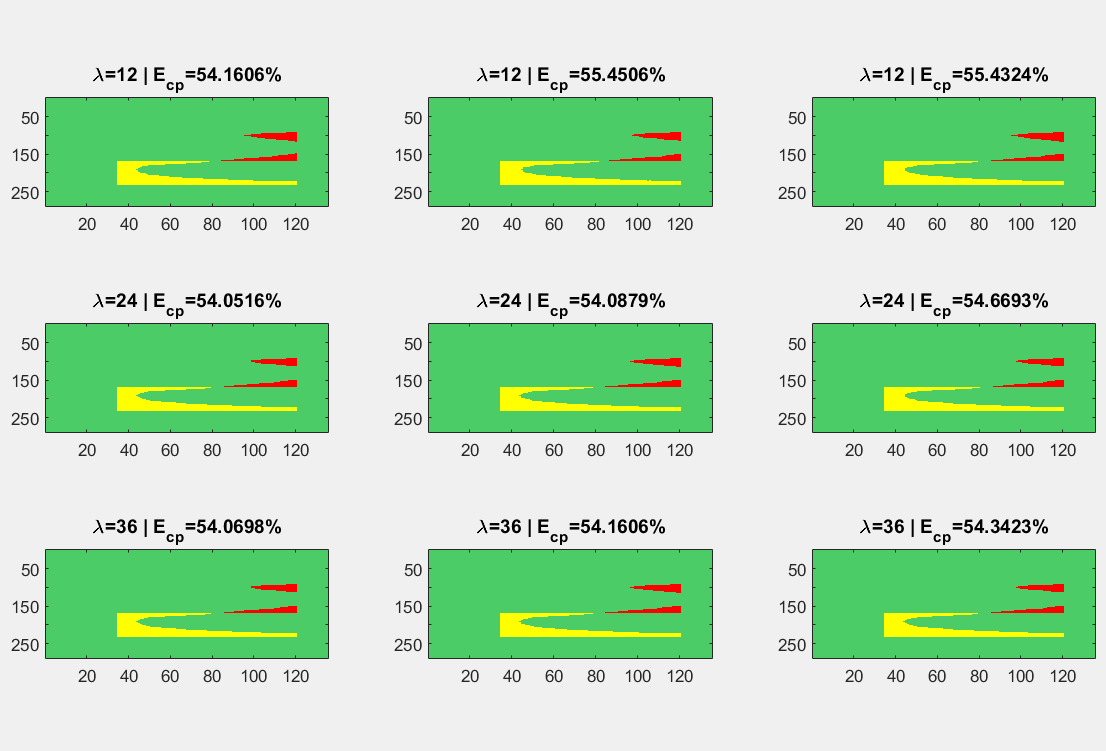
\includegraphics[width=7in]{figures/results_figures/lambda/cp_lambda_all.png}
\end{figure}
\\
Fig. \ref{fig:lambdaknobs}. shows that the knobs have very different behaviors between the executions with same $\lambda$ in terms of convergence time. We also observe that the convergence time increases with $\lambda$.\\
\begin{figure}[!h]
	\caption{[0-10] knobs history plots : non-unicity and evolution with $\lambda$.}
	\label{fig:lambdaknobs}
	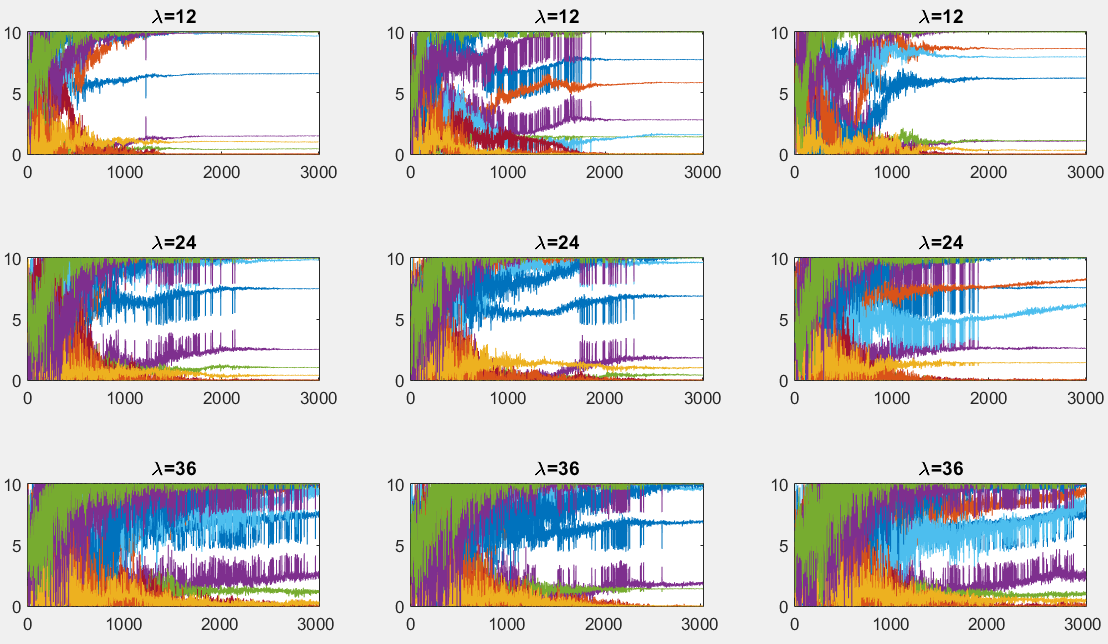
\includegraphics[width=7in]{figures/results_figures/lambda/knobs_lambda_all.png}
\end{figure}
\\
Fig. \ref{fig:lambdaknobsgenmean}. which is composed by [0-10] knob plots where the values for each BeATS evaluation have been replaced by the average value of their generation. It shows that the executions with same $\lambda$ converge to different knob values, whatever the $\lambda$. 
\begin{figure}[!h]
	\caption{[0-10] knobs "average of each generation" history plots : non-unicity and evolution with $\lambda$.}
	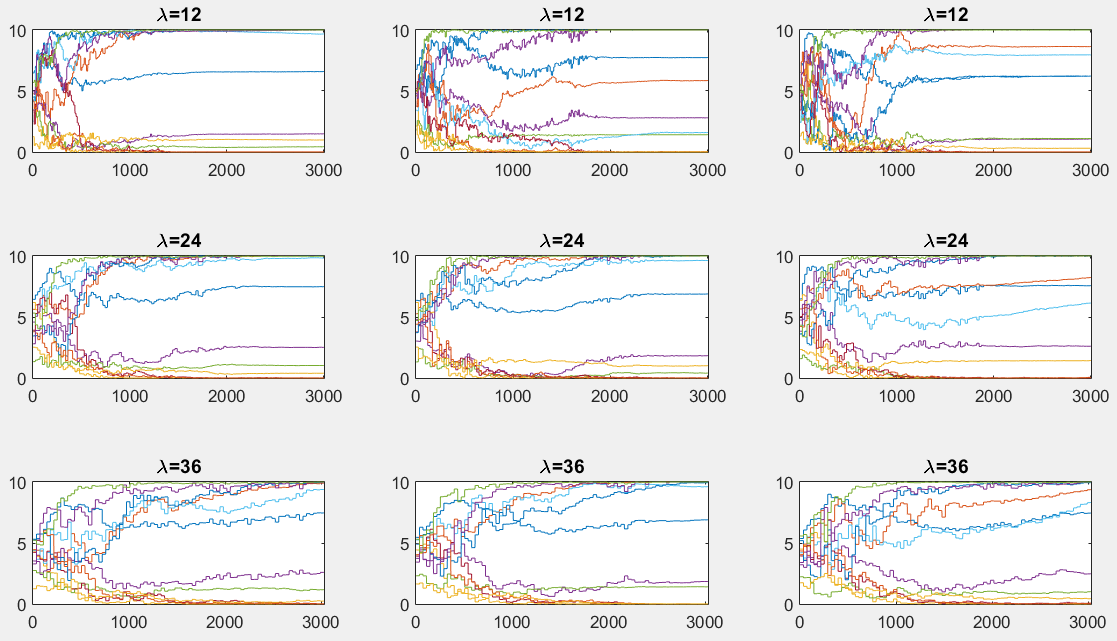
\includegraphics[width=7in]{figures/results_figures/lambda/knobs_lambda_all_genmean.png}
	\label{fig:lambdaknobsgenmean}
\end{figure}
\newpage
\emph{Conclusion:} The experiment allows the observation of the several equivalent global minima : the knobs converge to different values but to the same result quality. Our case does not empower us to highlight any influence of $\lambda$ on the result. It probably has when the search space dimension increases.